% Options for packages loaded elsewhere
\PassOptionsToPackage{unicode}{hyperref}
\PassOptionsToPackage{hyphens}{url}
%
\documentclass[
  english,
  man,floatsintext]{apa6}
\usepackage{amsmath,amssymb}
\usepackage{lmodern}
\usepackage{ifxetex,ifluatex}
\ifnum 0\ifxetex 1\fi\ifluatex 1\fi=0 % if pdftex
  \usepackage[T1]{fontenc}
  \usepackage[utf8]{inputenc}
  \usepackage{textcomp} % provide euro and other symbols
\else % if luatex or xetex
  \usepackage{unicode-math}
  \defaultfontfeatures{Scale=MatchLowercase}
  \defaultfontfeatures[\rmfamily]{Ligatures=TeX,Scale=1}
\fi
% Use upquote if available, for straight quotes in verbatim environments
\IfFileExists{upquote.sty}{\usepackage{upquote}}{}
\IfFileExists{microtype.sty}{% use microtype if available
  \usepackage[]{microtype}
  \UseMicrotypeSet[protrusion]{basicmath} % disable protrusion for tt fonts
}{}
\makeatletter
\@ifundefined{KOMAClassName}{% if non-KOMA class
  \IfFileExists{parskip.sty}{%
    \usepackage{parskip}
  }{% else
    \setlength{\parindent}{0pt}
    \setlength{\parskip}{6pt plus 2pt minus 1pt}}
}{% if KOMA class
  \KOMAoptions{parskip=half}}
\makeatother
\usepackage{xcolor}
\IfFileExists{xurl.sty}{\usepackage{xurl}}{} % add URL line breaks if available
\IfFileExists{bookmark.sty}{\usepackage{bookmark}}{\usepackage{hyperref}}
\hypersetup{
  pdftitle={What are the effective features of consultation: a mixed methods analysis},
  pdfauthor={Patrick Langford1, Tom Connor1, \& Andrew Tolmie1},
  pdflang={en-EN},
  pdfkeywords={Consultation, efficacy, evidence-based practice},
  hidelinks,
  pdfcreator={LaTeX via pandoc}}
\urlstyle{same} % disable monospaced font for URLs
\usepackage{longtable,booktabs,array}
\usepackage{calc} % for calculating minipage widths
% Correct order of tables after \paragraph or \subparagraph
\usepackage{etoolbox}
\makeatletter
\patchcmd\longtable{\par}{\if@noskipsec\mbox{}\fi\par}{}{}
\makeatother
% Allow footnotes in longtable head/foot
\IfFileExists{footnotehyper.sty}{\usepackage{footnotehyper}}{\usepackage{footnote}}
\makesavenoteenv{longtable}
\usepackage{graphicx}
\makeatletter
\def\maxwidth{\ifdim\Gin@nat@width>\linewidth\linewidth\else\Gin@nat@width\fi}
\def\maxheight{\ifdim\Gin@nat@height>\textheight\textheight\else\Gin@nat@height\fi}
\makeatother
% Scale images if necessary, so that they will not overflow the page
% margins by default, and it is still possible to overwrite the defaults
% using explicit options in \includegraphics[width, height, ...]{}
\setkeys{Gin}{width=\maxwidth,height=\maxheight,keepaspectratio}
% Set default figure placement to htbp
\makeatletter
\def\fps@figure{htbp}
\makeatother
\setlength{\emergencystretch}{3em} % prevent overfull lines
\providecommand{\tightlist}{%
  \setlength{\itemsep}{0pt}\setlength{\parskip}{0pt}}
\setcounter{secnumdepth}{-\maxdimen} % remove section numbering
% Make \paragraph and \subparagraph free-standing
\ifx\paragraph\undefined\else
  \let\oldparagraph\paragraph
  \renewcommand{\paragraph}[1]{\oldparagraph{#1}\mbox{}}
\fi
\ifx\subparagraph\undefined\else
  \let\oldsubparagraph\subparagraph
  \renewcommand{\subparagraph}[1]{\oldsubparagraph{#1}\mbox{}}
\fi
% Manuscript styling
\usepackage{upgreek}
\captionsetup{font=singlespacing,justification=justified}

% Table formatting
\usepackage{longtable}
\usepackage{lscape}
% \usepackage[counterclockwise]{rotating}   % Landscape page setup for large tables
\usepackage{multirow}		% Table styling
\usepackage{tabularx}		% Control Column width
\usepackage[flushleft]{threeparttable}	% Allows for three part tables with a specified notes section
\usepackage{threeparttablex}            % Lets threeparttable work with longtable

% Create new environments so endfloat can handle them
% \newenvironment{ltable}
%   {\begin{landscape}\begin{center}\begin{threeparttable}}
%   {\end{threeparttable}\end{center}\end{landscape}}
\newenvironment{lltable}{\begin{landscape}\begin{center}\begin{ThreePartTable}}{\end{ThreePartTable}\end{center}\end{landscape}}

% Enables adjusting longtable caption width to table width
% Solution found at http://golatex.de/longtable-mit-caption-so-breit-wie-die-tabelle-t15767.html
\makeatletter
\newcommand\LastLTentrywidth{1em}
\newlength\longtablewidth
\setlength{\longtablewidth}{1in}
\newcommand{\getlongtablewidth}{\begingroup \ifcsname LT@\roman{LT@tables}\endcsname \global\longtablewidth=0pt \renewcommand{\LT@entry}[2]{\global\advance\longtablewidth by ##2\relax\gdef\LastLTentrywidth{##2}}\@nameuse{LT@\roman{LT@tables}} \fi \endgroup}

% \setlength{\parindent}{0.5in}
% \setlength{\parskip}{0pt plus 0pt minus 0pt}

% \usepackage{etoolbox}
\makeatletter
\patchcmd{\HyOrg@maketitle}
  {\section{\normalfont\normalsize\abstractname}}
  {\section*{\normalfont\normalsize\abstractname}}
  {}{\typeout{Failed to patch abstract.}}
\patchcmd{\HyOrg@maketitle}
  {\section{\protect\normalfont{\@title}}}
  {\section*{\protect\normalfont{\@title}}}
  {}{\typeout{Failed to patch title.}}
\makeatother
\shorttitle{What are the effective features of consultation?}
\keywords{Consultation, efficacy, evidence-based practice\newline\indent Word count: X}
\usepackage{lineno}

\linenumbers
\usepackage{csquotes}
\usepackage{pdflscape}
\newcommand{\blandscape}{\begin{landscape}}
\newcommand{\elandscape}{\end{landscape}}
\ifxetex
  % Load polyglossia as late as possible: uses bidi with RTL langages (e.g. Hebrew, Arabic)
  \usepackage{polyglossia}
  \setmainlanguage[]{english}
\else
  \usepackage[main=english]{babel}
% get rid of language-specific shorthands (see #6817):
\let\LanguageShortHands\languageshorthands
\def\languageshorthands#1{}
\fi
\ifluatex
  \usepackage{selnolig}  % disable illegal ligatures
\fi
\newlength{\cslhangindent}
\setlength{\cslhangindent}{1.5em}
\newlength{\csllabelwidth}
\setlength{\csllabelwidth}{3em}
\newenvironment{CSLReferences}[2] % #1 hanging-ident, #2 entry spacing
 {% don't indent paragraphs
  \setlength{\parindent}{0pt}
  % turn on hanging indent if param 1 is 1
  \ifodd #1 \everypar{\setlength{\hangindent}{\cslhangindent}}\ignorespaces\fi
  % set entry spacing
  \ifnum #2 > 0
  \setlength{\parskip}{#2\baselineskip}
  \fi
 }%
 {}
\usepackage{calc}
\newcommand{\CSLBlock}[1]{#1\hfill\break}
\newcommand{\CSLLeftMargin}[1]{\parbox[t]{\csllabelwidth}{#1}}
\newcommand{\CSLRightInline}[1]{\parbox[t]{\linewidth - \csllabelwidth}{#1}\break}
\newcommand{\CSLIndent}[1]{\hspace{\cslhangindent}#1}

\title{What are the effective features of consultation: a mixed methods analysis}
\author{Patrick Langford\textsuperscript{1}, Tom Connor\textsuperscript{1}, \& Andrew Tolmie\textsuperscript{1}}
\date{}


\affiliation{\vspace{0.5cm}\textsuperscript{1} Institute of Education UCL}

\abstract{
Consultation is an integral part of many Educational Psychologist's (EPs) work. Yet there is a large heterogeneity in understanding and use of this tool. Such diversity makes evaluating its efficacy difficult. This research therefore sought to identify what the effective features of consultation are by linking observed features to changes in agreed outcomes for children and young people (CYP).
Mixed methods were employed to explore what EPs believe are the key features of consultation, what the barriers to effective consultation are, what happens in a consultation for a CYP, and what combination of features can be identified in consultations which lead to positive changes for CYP. To explore EP views towards the effective features of consultation, 30 EPs were interviewed. Observable features of consultation were tallied for six consultations. For those consultations, goals were identified by participants and a baseline rating was given for each goal using Target Monitoring Evaluation (TME) forms. There were 10 goals identified. Change for these goals was recorded through completing the same form 6-8 weeks later, to allow analysis of which combination of features were present for children with differing progress towards outcomes. This was assessed using Qualitative Comparative Analysis (QCA).
The most effective features of consultation, as identified by EPs, included the expert knowledge EPs have, the collaborative nature of consultation, and creating a shared understanding of the CYP and context for all participants. Consultations which were most likely to see positive change for the CYP were ones in which the consultation was not dominated by gaining an understanding of the presenting problem.
These results give clarity as to what the features of an effective consultation are. The findings have implications for EPs who use consultation, as well as consultees and those whom consultations are for.
}



\begin{document}
\maketitle

\hypertarget{introduction}{%
\section{Introduction}\label{introduction}}

Most Educational Psychology Services (EPS) in the U.K. have moved towards a predominantly consultation-based service (O'Farrell \& Kinsella, 2018). The most commonly employed consultation framework in the U.K. is the Wagner model (Wagner, 2000, 1995a, 1995b). It is defined as ``a voluntary, collaborative, non-supervisory approach, established to aid the functioning of a system and as inter-related systems'' (Wagner, 2000) through ``purposeful {[}conversations{]} which {[}use{]} techniques of listening, clarifying, problem-solving, challenging, questioning and reflecting'' (Munro, 2000). As a result, EPs work with those closest to the CYP, but not as experts telling those directly involved with the CYP how to help them. Their role is to help empower the consultees to solve their own problems in school. The focus is not only on the CYP but their relations with others and the many different environments they are in, such as home, school, and their wider community, ideas derived from Bronfenbrenner (1981).

Consultation is considered a form of `indirect' work as the theory is that the EP can enact the most change for the CYP by meeting and working with those around the CYP (Gutkin \& Conoley, 1990). Whilst this approach is highly prevalent, there is a large heterogeneity in practice. This can lead to a lack of understanding of what consultation is, by both EPs and consultees, as well as making it difficult to evaluate its efficacy. Given the need of EPs to demonstrate the efficacy of their work (Fallon et al., 2010), this poses serious problems for their ability to work in an ethical and effective manner. This is against the backdrop of EPs working within `traded services' (Lee \& Woods, 2017), where the ability to demonstrate efficacy is highly valued to ensure schools buy EP time again. It therefore behooves EPs to gain an understanding of the consistent features of consultation, so an attempt to assess the efficacy of it can be made

\hypertarget{features-of-consultation}{%
\subsection{Features of consultation}\label{features-of-consultation}}

Several pieces of work have previously attempted to identify the core features of consultation. One such paper (Kennedy et al., 2009) found that the most common behaviours by EPs were working
collaboratively, typically with those most involved (predominantly
parents) using either Solution-Focused approaches or problem-solving
analysis. Solution-Focused approaches are characterised by greater
interest in the solutions to presenting problems rather than the problem
itself. It views the client as capable of solving their own problems
with a changed mindset, facilitated by the EP, through identifying times
when the severity of the problem is reduced or it is not present, termed
`exceptions' (Rhodes \& Ajmal, 2004). Problem-solving
analysis is related to behavioural consultation
(Bergan \& Kratochwill, 1990) and is divided into four
stages: problem identification, problem analysis, treatment
implementation, and treatment evaluation
(Sheridan et al., 2000). Those working directly with the young
person, such as teachers, are involved throughout.

Similar results were found by Henderson (2013), who reported that the
mostly commonly given features of consultation were: discussing issues
with relevant parties; information gathering; and it being a reflexive
process with a focus on collaboratively crafting solutions. Nolan and Moreland (2014) details several key themes relating to the features of consultation. These were: empowering those involved in
the consultation; working collaboratively; the importance of each
participant in the consultation recognising the valuable knowledge from
others; reviewing outcomes; and EPs using their expertise to support
others (without emphasising their role as the ``expert''). O'Farrell and Kinsella (2018) found teachers appreciated
consultation as they felt empowered to support the pupils who had been
referred. According to Jones and Frederickson (1990), this
empowering of consultees rather than fixing the consultees problems or
simply giving advice, is part of the definition of consultation.

This research builds on a previous piece of work by the lead researcher.
This first work explored what EPs believe the key features of a
consultation are and what happened in an initial consultation between at
least an EP and a school staff member. This was done through a novel
questionnaire asking EPs to rank features of consultation according to
their importance and thematically analysing transcripts of
consultations. During the consultations, the two most frequent features
of consultation were `Understanding the presenting problem' and `Working
together to come up with solutions.' EPs rated these as core features of
consultation in the questionnaire, as well as improving outcomes for
young people.

To gain an understanding of what EPs at different LAs understood
consultation to be, the Local Offer literature was examined. This
information was found on the LA's websites and detailed what services
the EPS provided. Despite almost all services having moved to a
consultation-based service delivery
(Dinkmeyer \& Carlson, 2016), over a third of LAs did
not explicitly mention consultation. Of those that did, the most
commonly cited feature was working with relevant parties, such as
teachers. The second most common was improving outcomes for the CYP,
with the importance of looking for solutions (including the use of
Solution-Focused approaches) also being mentioned frequently. What this
shows is that for the LAs that mention it, the EPs working there have
explicitly stated the importance of collaborating with those closest to
the CYP and the necessity of improving the CYP's outcomes.

Although these studies typically only focused on a small number of
participants, the consistency in results allows fundamental features of
consultation to be gleaned. The studies also cover a wide range of EPS,
so the results are not limited to a specific region. This increases the
generalisability of the findings. However, despite these consistencies,
there is still a great deal of heterogeneity in consultation models and
practice. EPs can state they are engaging in consultation, but without
more information or a previously established working relationship, those
involved (parents, teachers, etc.) are unlikely to know what to expect
with a consultation. An arguably more serious consequence is that
assessing the efficacy of consultation is very difficult. If
consultations are not ergodic due to the very wide range of features,
any assessment of consultation may not be valid for consultations
performed by an individual EP. Therefore, assessing the efficacy of
consultations is difficult. This is against the backdrop of EPs working
within `traded services' (Lee \& Woods, 2017), where the
ability to demonstrate efficacy is highly valued. It therefore behooves
EPs to gain an understanding of the consistent features of consultation.
This will allow some assessment of which combination of features are
sufficient to lead to improved outcomes for CYP.

\hypertarget{evaluation-of-consultation}{%
\subsection{Evaluation of consultation}\label{evaluation-of-consultation}}

There have been calls for assessing the efficacy of EP work for decades, for example Cline (1994). Several tools have been put forward to attempt to do so. One such tool is Target Monitoring Evaluation (Dunsmuir et al., 2009). Target Monitoring Evaluation (TME) involves the negotiated development of SMART
goals (specific, measurable, achievable, realistic, and time limited)
between the EP and the consultees. To examine the suitability of using
TME forms with consultations, Dunsmuir et al. (2009)
incorporated TME forms into the practice of eight assistant EPs in one
county and 13 EPs based in two Local Authorities. During the initial
consultation, after the goals had been decided upon, each participant
rated how far along on a 10-point scale the child currently was towards
each goal. They then stated how far they expected the child to be when
they had their review consultation. 6-8 weeks later, during the review
consultation, each participant rated how far the child had actually
progressed, which was compared with how far they were predicted to
progress. Interviews were conducted with teachers, SENCOs, and
headteachers, who gave positive feedback on the easy and efficiency of
the process, as well as how the tool helped focus on setting of targets.

There have been a few studies which have attempted to compare TME with
other quantitative measures of change, such as
Connor (2010). In this thesis, the author
compared TME with other, more established forms of progress measurement
in domains like reading, such as the York Assessment of Reading
Comprehension (YARC). They report that there was broad agreement between
the TME and other forms of assessment; when other forms of assessment
found improvement, this was reflected in the reported change through the
TME forms.

\hypertarget{research-questions}{%
\subsection{Research questions}\label{research-questions}}

The general aim of this
research was to identify, through observations and interviews, what the key
features of consultations that lead to change for CYP are. This was done by
asking EPs what they believed the effective features of consultation are, what
makes them effective, and then observing consultations and systematically
noting which features occurred. This allowed the comparison of said features
with progress towards agreed goals for various CYP and whether they
reflected the views of EPs. As such, the research questions (RQs) were

\begin{enumerate}
\def\labelenumi{\arabic{enumi}.}
\item
  What are the core features of an effective consultation?

  \begin{enumerate}
  \def\labelenumii{\roman{enumii})}
  \item
    What do EPs believe are the key features of an effective
    consultation?
  \item
    What do EPs believe are the barriers to effective consultation?
  \item
    What do EPs believe makes those features effective?
  \end{enumerate}
\item
  Which combination of features of consultation are seen with progress
  towards agreed goals?
\end{enumerate}

\hypertarget{methods}{%
\section{Methods}\label{methods}}

All methods and results can be accessed at: \url{https://osf.io/6px7q/}.

\hypertarget{participants}{%
\subsection{Participants}\label{participants}}

Ethical approval was obtained from UCL the Institute of Education's
Ethical Committee. The inclusion criteria for both arms of the research
was: an EP or TEP who used consultation as part of their practice. There
were no requirements as to how frequently or recently it had to be used,
nor experience or location. Nor were there requirements around the
definition of consultation, just that EPs believed themselves to be
engaging in consultation.

For the interview and observation, participants were recruited via the researcher's EPS. Participants were also recruited to the interview by sharing calls for participants on a popular
mailing list for EPs and other education professionals (EPNET) and
social media (Twitter). Participants were also asked to share the call
for participants with other EPs at their work. Thus, a mixture of
convenience and snowball sampling (Robson \& McCartan, 2015) was
employed for the two arms of the research.

30 EPs of all roles and across the U.K. and Republic of Ireland were interviewed. 6 consultations were observed for 4 children. Child 1 had a joint home-school consultation, child 2 had one parent consultation and one school consultation, child 3 had one parent consultation, and child 4 had one school consultation and one parent consultation.

\hypertarget{material}{%
\subsection{Material}\label{material}}

\hypertarget{interviews}{%
\subsubsection{Interviews}\label{interviews}}

A semi-structured interview format was used because an interview
schedule was developed (Appendix 1) which served as a checklist of areas
to be explored with a given question order and wording. However, the
order and wording were allowed to change given the flow of the
interview. Additional questions were used to further develop an
interviewee's answer (Robson \& McCartan, 2015). Interviews were
chosen because they allow the interviewee to explain in detail their
thoughts and were judged to be the suitable means to explore the first
RQ. EPs have the greatest knowledge about consultation and are thus in
the best position to be able to explain what the effective features of
it are.

The interviews were of the focused type as the questions centred around
the key theme of consultation (Merton et al., 1990). The
core of this theme related to why EPs use consultation, what EPs believe
the key features of consultation are, why they are effective, what the
barriers to consultation are, and what is the unique contribution of
consultation. Barriers were explored because exploring this can help
reveal what the effective features of consultation are as often barriers
are a lack of an effective feature or the opposite of an effective
feature. The unique contribution of consultation was asked to further
explore what EPs believe makes consultation effective.

Probes (interview devices to elicit more information) were employed by
the researcher to further develop the interviewee's responses. To
achieve this, `laddering questions' (questions phrased in a variety of
ways asking for the interviewee to expand on their answer) and
`summarising techniques' (summarising what has just been said by the
interviewee to prompt more information), as well as `addition probes' to
maintain the flow of the conversation
(Zeisel \& Eberhard, 2006).

\hypertarget{observations}{%
\subsubsection{Observations}\label{observations}}

The quantitative arm of the research involved systematic observations of
consultations between an EP and either the parent, class teacher, or
both. Thus, it was a naturalistic observation as the participants were
observed in their typical environment without any interference from the
researcher (Vigliocco, 2001). Observation was
chosen as it helps overcome the often-recorded discrepancy between what
people say they do and how they behave in the real-world. This has been
reported in such wide-ranging fields as smartphone use
(Andrews et al., 2015) to driving behaviours
(Kaye et al., 2018).

Systematic observation was chosen because of the previous research
identifying features of consultation. The researcher therefore judged
that all the relevant observable features had been identified prior to
data collection. These observable features were developed into a coding
scheme (see Appendix 2 for the definition of each feature) to identify
categories over the course of a set period of time. The categories were
defined and operationalised prior to data collection
(Croll, 1986). They were derived from the
relevant literature and were mutually exclusive. The categories were
limited to what was explicitly said because this would help reduce the
amount of interpretation needed for behaviours such as non-verbal
interactions. Models of consultation, such as Solution-focused and
problem-analysis, were broken down into their constituent observable
parts, such as exploring strengths and identifying exceptions. Commonly
cited concepts in the literature such as `collaborative' were split into
explicit examples of those concepts, such as Everyone's contributions
valued.

Event sampling was used as the absolute and relative frequency of events
was of interest (Robson \& McCartan, 2015). A sequence record was
also used to provide information as to the order in which the features
were seen, thus providing information about transitions
(Robson \& McCartan, 2015).

\hypertarget{tme}{%
\subsubsection{TME}\label{tme}}

TME involves the negotiated development of SMART
goals (specific, measurable, achievable, realistic, and time limited)
between the EP and the consultees. During the initial
consultation, after the goals had been decided upon, each participant
rated how far along on a 10-point scale the child currently was towards
each goal. They then stated how far they expected the child to be when
they had their review consultation. 6-8 weeks later, during the review
consultation, each participant rated how far the child had actually
progressed, which was compared with how far they were predicted to
progress.

Connor (2010)
In this thesis, the author
compared TME with other, more established forms of progress measurement
in domains like reading, such as the York Assessment of Reading
Comprehension (YARC). They report that there was broad agreement between
the TME and other forms of assessment; when other forms of assessment
found improvement, this was reflected in the reported change through the
TME forms.

\hypertarget{procedure}{%
\subsection{Procedure}\label{procedure}}

Semi-structured focused interviews were used to elicit EP views with regards to the core features of consultation, the features of an effective consultation, the barriers to effective consultation, and what is the unique contribution of consultation. Participants were interviewed using a mixture of phone and
video call technology. Data collection took place between 31/03/2020 and
28/05/2020. An anonymous transcript was made for every interview. The anonymous transcripts were analysed using thematic analysis (TA), a methodology explicated by Braun and Clarke (2006). This was done using the software
NVivo 12. A mixed TA approach (Fereday \& Muir-Cochrane, 2006) was
employed. This incorporates inductive and deductive TA. Inductive TA is
driven primarily by the data
(Boyatzis, 1998) and deductive TA is
theory-driven with codes derived from said theory
(Crabtree \& Miller, 1992).

Observations were conducted between 20/11/2020 and 14/01/2021. After
gaining informed consent from all participants, the researcher observed
the consultation unfold as normal. The researcher used the observation
schedule to mark when and how frequently different features occurred. As
each feature was observed during the observation, a 1 would be written
in the corresponding column of the observation schedule. This would
continue sequentially, with only one feature being recorded in each
column until the conclusion of the consultation. The features were then
summed.

Immediately after the conclusion of the consultation, the participants
(EP, school class teacher, and/or parent) were asked to collectively
identify 1-3 goals for the CYP to work towards. This was done using a
TME form which the EP introduced the participants to. Goals were
suggested by the consultees or by the EP (if the consultee was unable to
think of a suitable goal). It was then agreed by all participants.
Participants rated, on a scale of 1-10, where the CYP currently was
towards that goal (by writing the letter `B' for `baseline' next to the
number) and where they expected them to be in 6-8 weeks (by writing the
letter `E' by the number). In 6-8 weeks' time, participants would be
contacted by the researcher via email to rate how far along the CYP had
progressed towards that goal. This judgement was represented by the
letter `A' (for `actual') along the same rating scale.

After the consultation, contact was made via email with the consultees
after 6 weeks. This was because it was judged that this would give
enough time for the participants to respond within the 8-week window
recommended by TME (Connor, 2010). All
consultees responded within 8 weeks. For all but child 4, this period
fell over the Christmas holidays. The upper limit was therefore chosen
to give the children as great a time as possible in school receiving
support. A second national lockdown was announced prior to the start of
the spring term. All the children except child 3 remained in school
during this lockdown.

\hypertarget{data-analysis}{%
\subsection{Data analysis}\label{data-analysis}}

Thematic analysis (TA) was used to explore RQ1 and its sub RQs. TA, as proposed by Braun and Clarke (2006), involves 6 stages: familiarizing yourself with your data; generating initial
codes; searching for themes; reviewing themes; defining and naming
themes; and producing the report. Codes were instances of features of
consultation discussed by the participants as this was the first step in
`data reduction' (Miles \& Huberman, 1994) by organising it
into meaningful groups (Tuckett, 2005).

A thematic map of codes was created using TikZiT, an open-source project
for creating diagrams (Kissinger, 2019). This was to visually
represent all the codes and aid in the generation of themes.
Boyatzis (1998) defines a theme as a
pattern contained within one's data which summarises the observations
through description. This helps to interpret the explored phenomenon.
Semantic themes (that which is explicitly said) were found and analysed
(Boyatzis, 1998) with interpretation
of their significance and implications
(Patton, 1990). TA identified 32 inductive
codes, as well as the 15 deductive codes previously set, relating to
what features EPs believed were effective for consultation. 6 codes were
identified for what made said features effective (see Appendix 3 for the
definitions of the inductive codes, Appendix 4 for the definitions of
the codes relating to what makes the features effective and Appendix 5
for the breakdown of the number of interviews which each code was
identified in and the total number of codes for each feature). These
were combined to create 8 themes: Buy-in, Conditions, Context,
Strengths-based, Shared understanding, Intervention, Future facing, and
EP skills and knowledge. These could then be combined to create two
overarching themes: Internal factors (features relating to the factors
endemic to a consultation) and External factors (features relating to
things happening around a consultation).

For the quantitative arm of the research, 6 observations were conducted for 4 children. After the tabulation of
features of consultation using the observation schedule, the number of
features across each consultation was summed. Qualitative notes were
made on the demeanour and enthusiasm of the consultees. The data from
the TME forms for all goals was collected and a value of `change' was
calculated for each consultation. This was done by subtracting the
`baseline' rank from the `actual' as research suggests most TME forms
report a positive change as a result of the consultation
(Dunsmuir et al., 2009; Monsen et al., 2009).
To explore the relationship between the presence of features and
reported change, Qualitative Comparison Analysis (QCA) was used, with
the QCA package for R (Dușa, 2018). QCA allows
the comparison of cases with the ``help of formal tools and with a
specific conception of cases'' (Rihoux \& Lobe, 2009). However, due to there being more conditions than cases, conclusions from QCA cannot be drawn as each case formed a unique configuration, thus invalidating the ability of QCA to find common combinations (Marx \& Dusa, 2011).

\hypertarget{results}{%
\section{Results}\label{results}}

\hypertarget{qualitative}{%
\subsection{Qualitative}\label{qualitative}}

Given the large number of codes and themes identified, what follows will be an examination of two of the key themes within the overarching theme Internal factorsand one of the themes from External factors.

\begin{landscape}

\textbf{Figure 1}

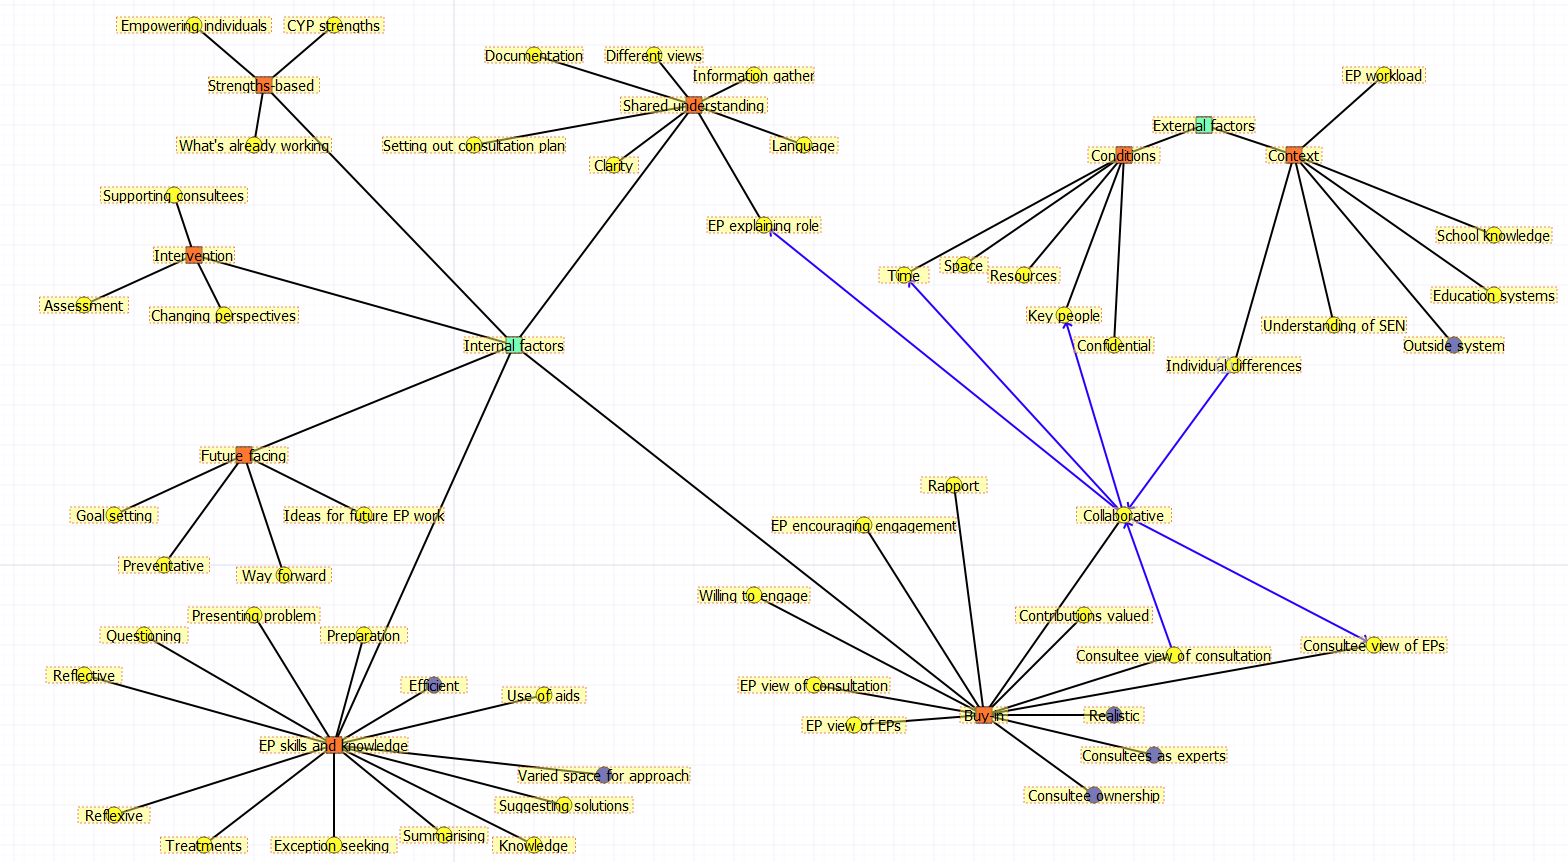
\includegraphics{Thematic_map.png}

\emph{Note.} Light blue square: over-arching theme, orange square: theme,
yellow circle: feature of consultation code, dark blue circle: what
makes the feature effective code, black line = connection from code to
theme to over-arching theme, blue line = connection between code (with
arrow pointing to direction of influence).

\end{landscape}

The thematic map of codes and features (see Figure 1) was derived from
analysing the codes for similarities around their nature to give themes
(Braun \& Clarke, 2006). For example, the essence of codes
such as `collaborative' and `contributions valued' related to the
consultees viewing the consultation as a good use of their time and
believing that it would lead to change for the CYP. This buy-in was
linked to the outcomes and suggestions from the consultation being
realistic, as consultees would be more likely to do what had been
suggested and believe it would have a positive impact. By treating the
consultee as an expert in their area of knowledge, this would help
increase their buy-in to the process of consultation and be more willing
to engage.

This collaborative nature of consultation was expressed by many participants, : \emph{``effective consultation shouldn't
being a meeting where one person dominates, whether that may be a
psychologist or anyone else''} (Interview 11) and \emph{``it's like we're all
involved, we're all at the same level, we just come at it from a
different perspective''} (Interview 7).

EP skills and knowledge was identified as many of the effective features
of consultation were related to the EP having expert knowledge of viable
solutions or through their understanding of psychological models. These
all increased the efficacy of consultation. Through EP skill with
regards to their expert knowledge and ability to ask questions, for
example, consultation could be an efficient means to enact change.
Consultation also allowed for EP skill to be shown by being a flexible
model of working, such that EPs could a wide range of their skills and
knowledge to help CYP.

The most common code across all themes was in relation to the models of
consultation and general psychological knowledge that the interviewees
believed EPs needed to have to facilitate an effective consultation. The
\emph{``use of theory and reference to the evidence base''} (Interview 2) was
identified as an important effective feature of consultation. Commonly
discussed models and frameworks included being solution-focused
(Interview 1), person-centred (Interview 16), trauma and attachment
informed (Interview 13), and using Wagner's model of consultation
(Interview 17) and the COMOIRA model (Interview 25).

One of the main codes of the theme Condition was Key people. Almost every interviewee cited having \emph{``all the key stakeholders''}
(Interview 11) involved in the consultation as a key aspect.
Consultation was widely regarded as an \emph{``indirect service method''}
(Interview 17) so involved working with a range of people, including
\emph{``the SENCO, the class teacher, and both the mum and dad of that child''}
(Interview 11). Many interviewees state that it was crucial to have
\emph{``the person that has most knowledge about the child''} (Interview 10) or
the \emph{``people who are most concerned''} (Interview 21). This included the
person who \emph{``has the most influence''} (Interview 14) as they will be the
person who will implement the agreed interventions.

A number of interviewees highlighted the importance of bringing the
voice of the CYP into the consultation, either by actively involving
them in the consultation (Interview 21) or through those that know the
CYP well (Interview 15).

Many interviewees identified difficulties with conducting consultations
in secondary schools:

\begin{quote}
\emph{\ldots if you've got multiple people working with a young person, and
actually the more people you have, the less anybody feels any
responsibility for them\ldots{} you're trying to find that person who is
most concerned and actually they don't exist. (Interview 13)}
\end{quote}

\begin{quote}
\emph{\ldots it's very difficult to get parents, teachers, parents and teachers
around the same table, at the same time. (Interview 18)}
\end{quote}

\hypertarget{quantitative}{%
\subsection{Quantitative}\label{quantitative}}

Table 1 summarises the cumulative frequencies of each feature for each
consultation. The most frequently observed feature was Understanding the
presenting problem, followed by CYP strengths, and then Info gather. 3
features were observed on zero occasions (School knowledge, EP
explaining role, and Planning/implementing treatments). Understanding
the presenting problem was observed the most frequently in every
consultation, often twice as frequently as the next most observed
feature. CYP strengths was the next most frequently observed, followed
by Information gather.

\begin{landscape}

\textbf{Table 1}

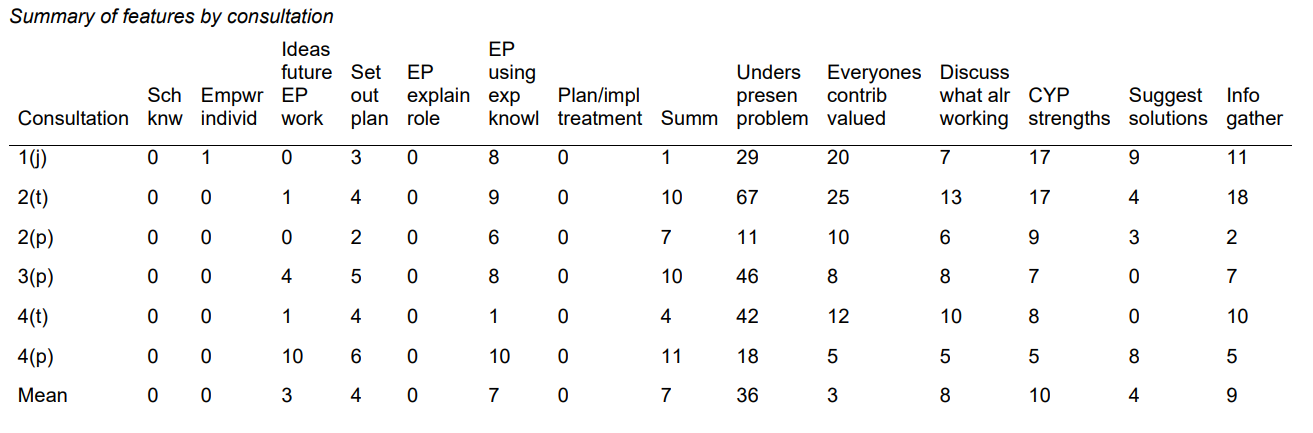
\includegraphics{Table_1.png}

\end{landscape}

\textbf{Table 2}

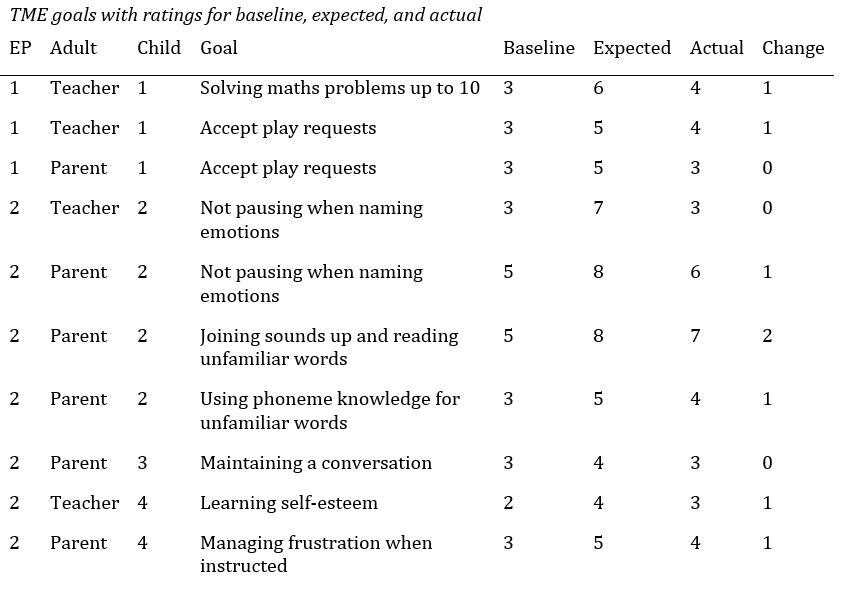
\includegraphics{Table_2.png}

\hypertarget{discussion}{%
\section{Discussion}\label{discussion}}

\hypertarget{rq-1.1-what-do-eps-believe-are-the-key-features-of-an-effective-consultation}{%
\subsection{RQ 1.1 What do EPs believe are the key features of an effective consultation?}\label{rq-1.1-what-do-eps-believe-are-the-key-features-of-an-effective-consultation}}

The 8 themes regarding the core features of consultation encapsulate a
very broad range of aspects of consultation that a number of EPs (of
varying levels of experience) believe are important for making
consultation effective. The most frequently identified themes were
Buy-in and EP skills and knowledge. There was a large disparity between
the number of inductive and deductive codes. There was also a difference
between the number of instances for each type of code, with the
inductive codes being recorded more frequently than deductive codes.
This suggests that the current literature does not accurately reflect
EP's beliefs about effective consultation.

\hypertarget{buy-in}{%
\subsubsection{Buy-in}\label{buy-in}}

Buy-in referred to all the participants of the consultation, including
the EP, believing that consultation is an effective method for enacting
change for the CYP in question. Believing that this was a valuable use
of their time and that it could help the CYP was believed by many
interviewees to be essential for an effective consultation. Without this
buy-in, consultees would not be willing to engage with the process or
change anything as a result of the consultation. And if nothing changed,
it is unlikely the situation would improve for the CYP, and it is even
less likely the EP could have a positive impact through consultation
(Noell \& Gansle, 2014).

This buy-in could be established at two time points: prior to the
consultation and during the consultation. Before the consultation, the
consultees view of consultation had a large impact on whether they
valued the process. If they understood what it was (via explanation or
training) and believed that it could help, then the chances of the
consultation having a positive impact improved. If they understood that
they were an active member of the consultation and did not look to the
EP as the expert who would fix the problem for them, then they could
buy-in to the process and an effective consultation was more likely to
occur. Hasselbusch and Penman (2008) found that
consultants being perceived as the expert was felt to have a limiting
impact on the efficacy of the consultation and many participants shared
this view. Buy-in was also facilitated by the EP not viewing themselves
as the expert who was there to tell the consultees what they needed to
do to solve the problem. Thus, prior to the consultation, buy-in for
both the consultees and EP could be established through these
mechanisms.

During the consultation, buy-in by those involved could be facilitated
by the EP. By being collaborative and actively involving the consultees
in the consultation, the EP could encourage their buy-in to the process.
By giving the consultees the opportunity to voice their opinions and
concerns and listening to them, this helped the consultees feel valued
and an active participant in the process
(Benn et al., 2008). Consultee voice has been
identified as crucial for effective consultation
(Newman et al., 2017) and these results
further substantiate this idea. These all served to help create a
rapport between the EP and consultees. This relationship was one of the
most important features of an effective consultation, as without a
trusting relationship between consultees and the EP, consultation cannot
be an effective vehicle for change (Meyers et al., 2014).
Rapport also formed the foundation for many of the ways consultation
helped consultees, such as through changing consultee perspectives. This
buy-in also greatly increases the chance of solutions being implemented,
which is one of the main mechanisms through which consultation creates
positive change (Meyers et al., 2014).

\hypertarget{ep-skills-and-knowledge}{%
\subsubsection{EP skills and knowledge}\label{ep-skills-and-knowledge}}

This theme related to all the ways that EPs use the knowledge gained
over the course of their training and professional practice. It has been
argued that "{[}possessing{]} expert knowledge and skills in the field of
educational psychology theory and practice is one of, if not the, most
important requirement for effective consultation
(Farrell \& Woods, 2015). This is reflected in the
results, as every interviewee mentioned at least one example of expert
knowledge they used in their practice. In addition, many explicitly
talked about the importance of this knowledge for effective
consultation.

Specific examples of this knowledge included core models of
consultation, such as Patsy Wagner's model of consultation, as well as
Jey Monsen's Problem-analysis framework.
Meyers et al. (2014) argue that effective consultation
requires steps such as ``problem definition'' and other core parts of the
Monsen framework. Many interviewees cited the Problem-analysis framework
as their primary model and a core part of an effective consultation.
However, few interviewees stated they strictly held to any one model.
Many stated they used different elements from different models as and
when appropriate. This paints a picture of consultation, as used by EPs,
as an assortment of different skills and knowledge rather than strict
adherence to one method. To date, there has been no examination of the
efficacy between consultations when there is strict adherence to the
model versus a more eclectic mix. It is therefore unknown whether this
approach to consultation is as effective as strictly using a
consultation model.

Ideas from Solution-focused therapy were frequently mentioned, including
specific components such as the miracle question and looking for
exceptions. Other examples included using person-centred processes such
Narrative therapy. This was the only code to be cited by every EP yet
seems to run counter to the often-presented argument ``I am not the
expert.'' This may represent an epistemic conflict between EP's desire to
not be placed in a position of power for fear of undermining consultee
engagement, but also recognising the need to have expert knowledge to be
able to lead an effective consultation. One of the reasons it was
believed to be essential for effective consultation was because many
believed it formed the bedrock of how the EP leads a consultation. This
knowledge also helps provide a structure for the consultation, thus
making it more effective (Wagner, 2008).
This is because a structure can help keep the consultation focused on a
single concern which can be tackled
(Newman et al., 2017).

The ability to ask difficult questions and to know what questions to ask
to move a situation forward were frequently given as a key feature of
effective consultation. These questions, developed through training and
experience, help identify the presenting problem and limits to this, as
well as areas where they need more information
(Hylander, 2017). By thoroughly
preparing for the consultation, for example having questions prepared in
advance, the efficacy of it can be increased. This is because it is
easier to know what questions to ask and to keep to the structure.
However, as some interviewees argued, keeping to the structure should
not come at the expense of listening to the concerns of the consultees
and being flexible to their needs. Without this, consultees risk feeling
devalued and thus disengaging
(Slonski-Fowler \& Truscott, 2004). This presents another
difficulty for EPs who wish to use consultation effectively. Whilst this
psychological knowledge is viewed as essential for effective
consultation, it can undermine this method by being too rigid.

\hypertarget{rq1.2-what-do-eps-believe-are-the-barriers-to-effective-consultation}{%
\subsection{RQ1.2 What do EPs believe are the barriers to effective consultation?}\label{rq1.2-what-do-eps-believe-are-the-barriers-to-effective-consultation}}

The barriers to effective consultation were examined because through the
exploration of factors which undermine the efficacy of consultation, it
will reveal what is needed for an effective consultation to occur. Two
of the biggest barriers brought up by interviewees were not having the
key people involved or not having sufficient time. For a consultation to
be effective, the people who are in a position to change things need to
be involved. If they are not, they are unlikely to buy-in to the
proposed change and make sure it happens. The efficacy of the
consultation is also reduced if one is trying to elucidate a situation
and someone who knows the CYP is not present. Therefore, having the key
people as part of the consultation is essential for it to reach its full
potential of providing clarity and changing the situation (through
perspective change and identifying support strategies).

Time constraints was identified as one of the main barriers to effective
consultation. Therefore, an effective consultation needs time. The
minimum time limit for an effective consultation was judged to be 30
minutes, although most interviewees preferred to have 45 minutes to one
hour. This meant that the consultees did not feel rushed through the
process, which undermines the efficacy of consultation
(Webster et al., 2003). Having time also ensures
that consultees could be properly supported emotionally before exploring
solutions. Time has also been found to be essential for consultee
empowerment and learning (D. M. Truscott \& Truscott, 2004). A
lack of time has also been found to decrease the consultee's sense of
ownership for the solutions (Babinski \& Rogers, 1998), which
is one of the main mechanisms through which the features of consultation
are effective (see section 5.1.1.3).

A perennial barrier to effective consultation is a lack of resources
from the school. If the school do not have the resources to implement
any of the devised solutions, it is unlikely the situation will improve
for the CYP. This lack of resources may also affect the consultees as
they feel disempowered even before they have entered the consultation.
They are therefore less likely to buy-in to the process of actively
seeking change and taking ownership of the situation, because they feel
like forces beyond their control are stopping them.

\hypertarget{rq-1.3-what-do-eps-believe-makes-those-features-effective}{%
\subsection{RQ 1.3 What do EPs believe makes those features effective?}\label{rq-1.3-what-do-eps-believe-makes-those-features-effective}}

The most frequently discussed reason that the identified features help
ensure consultation is effective is that it is efficient. This took a
few forms, such as being efficient for seeing more children in a short
space of time (as opposed to direct work with children). Many of the
benefits reflect some of the pressure's interviewees felt. Several EPs
discussed the need to use consultation because schools could not buy in
more time but wanted psychological input for a large number of children.
They may have also perceived a need to demonstrate their value for money
within a traded context (Lee \& Woods, 2017) and so
emphasised the cost-efficient nature of consultation. However,
consultation was also efficient because of its ability to have an impact
wider than the consultation itself. Through empowering consultees,
changing perspectives, and emotionally supporting consultees,
consultation can have positive effects for consultees, CYP, and schools
as a whole if they change policy as a result of an effective
consultation.

The key reason identified for making such features as Collaborative, EP
encouraging engagement, and Rapport effective was the fact it engendered Consultee
ownership of the situation. By making the consultation Collaborative, by
Empowering consultees, those involved feel better equipped to support
the CYP and more motivated to implement recommendations
(Erchul \& Martens, 2012).

A number of interviewees talked about the importance of being external
to the school system. This being outside the school system meant that
questions could be asked that otherwise could not be and an external
perspective could be brought in
(Cording, 2011). This is particularly
valuable for when a situation feels ``stuck,'' and consultees feel
powerless. By being external, they may be able to see what is already
working and give new recommendations for supporting the CYP.

The giving of recommendations links to another mechanism through which
these features of consultation are effective: that what is recommended
is Realistic. By listening to the consultees and valuing their opinions,
EPs are more likely to be able to make recommendations that fit within
the context of the school and can be reasonably put in. If an EP makes a
series of grand recommendations for the CYP but the school do not have
the means to implement them, then there is little chance the situation
will improve. But by having a collaborative consultation, in which
recommendations are co-created, the solutions are more likely to be
feasible and therefore the chance of having an effective consultation
and a positive impact is increased. This is associated with the final
mechanism through which these features are effective: treating the
Consultees as experts. By taking on board the views of the consultees
and seeing them as having expertise to bring to the discussion, the
consultation is more likely to be effective
(S. Truscott et al., 2012). Consultees will be more likely
to buy-in to the process if they feel valued and listened to and the
recommendations are more likely to be relevant if those who know the
school and CYP most are actively involved. Whilst there is theoretical evidence to suggest this an important feature, only a small number of interviewees explicitly
mentioned this as a valuable mechanism for effective consultations. This reveals another instance of the disparity between what the academic literature highlights as important and what practicing EPs believe is important.

\hypertarget{rq-2-which-combination-of-features-of-consultation-are-seen-with-progress-towards-agreed-goals}{%
\subsection{RQ 2 Which combination of features of consultation are seen with progress towards agreed goals?}\label{rq-2-which-combination-of-features-of-consultation-are-seen-with-progress-towards-agreed-goals}}

A majority of the goals were judged to have experienced progress,
bolstering the claim made in Dunsmuir et al. (2009). Of
those which saw progress, patterns can be drawn. A qualitative
examination of the correspondence between features of consultation and
change revealed that consultations with fewer recorded instances of
Understanding the presenting problem were more likely to see change.
Such examples include the parent consultation for child 2 and the parent
consultation for child 4 (see Appendix L for all observed features and
change). There was also a greater number of instances of Suggesting
solutions by the EP during consultations which saw change, such as the
first consultation and the parent consultation for child 4.

There was a disparity between what interviewees stated was important and
what was observed in the consultations. Collaboration was given by
almost every interviewee as a crucial feature. However, observable
instances of this feature were less frequently seen than the EP
exploring the presenting problem for a majority of consultations. This
may represent a gap between what EPs say is important and what they
do in a consultation when they are there to support a specific
CYP in that context. It does, however, corroborate the importance of EPs
using parts of models e.g., the Problem-analysis framework. This is
because for each consultation the most frequently seen feature was
Understanding the presenting problem. This is substantiated by the fact
one of the EPs who was observed stated in their interview that the main
model they use in their practice is the Problem-analysis framework. On
the other hand, this emphasis on exploring the depth and limits of the
main problem may not reflect adherence to this model (and thus be
evidence for the importance of using said model). It may just be an
exploration of the main difficulties (and arguably the reason why the
consultation was organised in the first place). The absence of other
features of the Problem-analysis framework, such as discussing how to
implement an intervention, is suggestive of the perceived need by EPs to
fully understand the presenting problem rather than fully commit to a
certain model. This suggests a disparity between how EPs say they work
and what happens in a consultation.

The importance of the individual differences of the consultees was
highlighted in these observations, as consultees who were more
optimistic and less stressed were better able to engage collaboratively
and not focus as much on exploring the negative aspects of the
situation. Examples of these include the parent consultation for child 2
as the ratio between Understanding presenting problem and other features
was more even. The teacher consultation for child 2 was also an
opportunity to highlight the importance of emotionally supporting
consultees, given how upset the consultee was and therefore unable to
engage with one aspect of the consultation prior to said support.

The fact three putatively core features of effective consultation
(School knowledge, EP explaining role, and Planning/implementing
treatments) were not recorded once undermines the argument that they are
important for effective consultations. This is also true for Empowering
individuals as this was only recorded once. They do not appear to be
necessary and perhaps are not sufficient for change to be judged as
having occurred. Even though there were instances of the EP offering
solutions in most consultation, there was no discussion of the specifics
of how any suggestion was to be implemented (as there were no recorded
instances of Planning/implementing treatments). There was also no review
of any prior treatments. This raises questions as to how effective the
suggestions are. If they are left to the consultees to establish and
decide how often an intervention should be run for, will it be as
effective as if it were decided with the person who is believed to have
expert knowledge?

There was a lack of consistency regarding the discrepancy between the
ratings given by parents and teachers: one consultation saw the teacher
identifying change and the parent not, another saw the parent judging
there to have been progress but the teacher not. This reflects the fact
TME is based upon the perceptions of change by consultees and thus there
may be different conceptions and criteria for judging change between
consultees (Connor, 2010). However, the sample
is too small to draw any patterns or conclusions from this data.

\hypertarget{conclusions}{%
\section{Conclusions}\label{conclusions}}

This piece of work represents an attempt to systematically identify the
features of consultation which lead to change for CYP. By employing a
mixed methods approach, the beliefs of practicing EPs regarding the
effective features of consultation were detailed, along with recorded
instances of various features of consultation. These recordings were
tabulated against measures of change for co-operatively agreed goals by
the EP and consultees. The relative presence or absence of said features
were then analysed to see if patterns of features could be identified.
Whilst statistical analyses did not yield conclusive results, the
breadth of qualitative data combined with the non-formal analysis of
features and ratings of change present a picture of what is necessary
for an effective consultation.

To lead an effective consultation, EPs need to have specialist knowledge
to thoroughly explore an area of need for a child or young person. By
creating a collaborative space in which consultees feel valued, through
the development of rapport and encouraging the participation of
consultees, EPs can hope to change the perspectives of those involved
and identify potential solutions. By exploring the views of consultees
and using various questions, a shared understanding of the CYP and
situation can be created. Through consultation, EPs can impact not only
those involved in the consultation, by providing therapeutic support,
but those outside the consultation through the ripple effects
consultation can have on people and systems. By being collaborative,
consultees can not only feel empowered to support CYP but to take
ownership of the situation and actively work to improve the situation
for all.

Consultation is fundamental to the work of EPs in the U.K. Yet there remain significant questions as to what
constitutes consultation and how it can be effective in supporting CYP.
This presents great challenges to TEPs and EPs alike, resulting in many
claiming to practice consultation when in fact they do not. It is
therefore of vital importance for us as a profession to clarify what we
mean by consultation and how we can engage in it effectively. My hope is
that this work can go some way in shining a light on the core features
of an effective consultation and thus empower EPs to lead consultations
which improve the lives of those we seek to help.

\newpage

\hypertarget{references}{%
\section{References}\label{references}}

\begingroup
\setlength{\parindent}{-0.5in}
\setlength{\leftskip}{0.5in}

\hypertarget{refs}{}
\begin{CSLReferences}{1}{0}
\leavevmode\hypertarget{ref-andrewsSelfReportToolsCompare2015a}{}%
Andrews, S., Ellis, D. A., Shaw, H., \& Piwek, L. (2015). Beyond {Self}-{Report}: {Tools} to {Compare Estimated} and {Real}-{World Smartphone Use}. \emph{PLOS ONE}, \emph{10}(10), e0139004. \url{https://doi.org/10.1371/journal.pone.0139004}

\leavevmode\hypertarget{ref-babinskiSupportingNewTeachers1998}{}%
Babinski, L. M., \& Rogers, D. L. (1998). Supporting new teachers through consultee-centered group consultation. \emph{Journal of Educational and Psychological Consultation}, \emph{9}(4), 285--308. \url{https://doi.org/10.1207/s1532768xjepc0904_1}

\leavevmode\hypertarget{ref-bennAnalysisInstructionalConsultants2008}{}%
Benn, A. E., Jones, G. W., \& Rosenfield, S. (2008). Analysis of instructional consultants' questions and alternatives to questions during the problem identification interview. \emph{Journal of Educational and Psychological Consultation}, \emph{18}(1), 54--80. \url{https://doi.org/10.1080/10474410701864115}

\leavevmode\hypertarget{ref-berganBehavioralConsultationTherapy1990}{}%
Bergan, J. R., \& Kratochwill, T. R. (1990). \emph{Behavioral {Consultation} and {Therapy}: {An Individual Guide}} (1990 edition). {Springer}.

\leavevmode\hypertarget{ref-boyatzisTransformingQualitativeInformation1998a}{}%
Boyatzis, R. E. (1998). \emph{Transforming qualitative information: Thematic analysis and code development}. {SAGE}.

\leavevmode\hypertarget{ref-braunUsingThematicAnalysis2006}{}%
Braun, V., \& Clarke, V. (2006). Using thematic analysis in psychology. \emph{Qualitative Research in Psychology}, \emph{3}(2), 77--101. \url{https://doi.org/10.1191/1478088706qp063oa}

\leavevmode\hypertarget{ref-bronfenbrennerEcologyHumanDevelopment1981}{}%
Bronfenbrenner, U. (1981). \emph{The {Ecology} of {Human Development}: {Experiments} by {Nature} and {Design}} (unknown edition). {Harvard University Press}.

\leavevmode\hypertarget{ref-clineQualityAssuranceEducational1994a}{}%
Cline, T. (1994). Quality {Assurance} in an {Educational Psychology Service}: {What Can We Learn} from {Earlier Experience} in {Service Evaluation}? \emph{School Psychology International}. \url{https://doi.org/10.1177/0143034394153002}

\leavevmode\hypertarget{ref-connorTargetMonitoringEvaluation2010}{}%
Connor, T. (2010). \emph{Target monitoring and evaluation : Measuring the impact of educational psychology interventions} {[}Ph.\{\{D\}\}.{]}. Institute of Education, University of London.

\leavevmode\hypertarget{ref-cordingStudyEducationalPsychologists2011}{}%
Cording, J. (2011). \emph{A study of {Educational Psychologists}' use of consultation and users' views on what a service should deliver}. 158.

\leavevmode\hypertarget{ref-crabtreeTemplateApproachText1992}{}%
Crabtree, B. F., \& Miller, W. F. (1992). A template approach to text analysis: {Developing} and using codebooks. In \emph{Doing qualitative research} (pp. 93--109). {Sage Publications, Inc}.

\leavevmode\hypertarget{ref-crollSystematicClassroomObservation1986}{}%
Croll, P. (1986). \emph{Systematic {Classroom Observation}}. {Routledge}.

\leavevmode\hypertarget{ref-dinkmeyerConsultationCreatingSchoolBased2016}{}%
Dinkmeyer, D., \& Carlson, J. (2016). \emph{Consultation: {Creating School}-{Based Interventions}} (4th edition). {Routledge}.

\leavevmode\hypertarget{ref-dunsmuirEvidenceBasedPractice2009}{}%
Dunsmuir, S., Brown, E., Iyadurai, S., \& Monsen, J. (2009). Evidence-based practice and evaluation: From insight to impact. \emph{Educational Psychology in Practice}, \emph{25}(1), 53--70. \url{https://doi.org/10.1080/02667360802697605}

\leavevmode\hypertarget{ref-dusaQCAComprehensiveResource2018}{}%
Dușa, A. (2018). \emph{{QCA} with {R}. {A Comprehensive Resource}}. \url{https://doi.org/10.1007/978-3-319-75668-4}

\leavevmode\hypertarget{ref-erchulSchoolConsultationConceptual2012}{}%
Erchul, W. P. P., \& Martens, B. K. (2012). \emph{School consultation: Conceptual and empirical bases of practice} (2010th edition). Springer.

\leavevmode\hypertarget{ref-farrellReflectionsRoleConsultation2015}{}%
Farrell, P., \& Woods, K. (2015). Reflections on the role of consultation in the delivery of effective educational psychology services. \emph{Educational Psychology Research and Practice}, \emph{1}(1), 2--9.

\leavevmode\hypertarget{ref-feredayDemonstratingRigorUsing2006}{}%
Fereday, J., \& Muir-Cochrane, E. (2006). Demonstrating {Rigor Using Thematic Analysis}: {A Hybrid Approach} of {Inductive} and {Deductive Coding} and {Theme Development}. \emph{International Journal of Qualitative Methods}, \emph{5}(1), 80--92. \url{https://doi.org/10.1177/160940690600500107}

\leavevmode\hypertarget{ref-gutkinReconceptualizingSchoolPsychology1990}{}%
Gutkin, T. B., \& Conoley, J. C. (1990). Reconceptualizing school psychology from a service delivery perspective: {Implications} for practice, training, and research. \emph{Journal of School Psychology}, \emph{28}(3), 203--223. \url{https://doi.org/10.1016/0022-4405(90)90012-V}

\leavevmode\hypertarget{ref-hasselbuschWorkingTogetherOccupational2008}{}%
Hasselbusch, A., \& Penman, M. (2008). Working Together: An Occupational Therapy Perspective on Collaborative Consultation. \emph{Kairaranga}, \emph{9}(1), 24--31. \url{http://eprints.bournemouth.ac.uk/9861/}

\leavevmode\hypertarget{ref-hendersonExplorationImpactConsultation2013}{}%
Henderson, A. (2013). \emph{An exploration of the impact of consultation on educational psychology service users, namely teachers, parents and pupils in a large rural local authority} {[}Ed.\{\{Psych\}\}.\{\{D\}\}.{]}. University of Birmingham (United Kingdom).

\leavevmode\hypertarget{ref-hylanderEstablishingPsychologicalConsultation2017}{}%
Hylander, I. (2017). \emph{Establishing Psychological Consultation Services to Promote Student Well-Being in Schools and Preschools} (1st ed.). Routledge. \url{https://www.taylorfrancis.com/https://www.taylorfrancis.com/chapters/edit/10.4324/9781315795188-2/establishing-psychological-consultation-services-promote-student-well-being-schools-preschools-ingrid-hylander}

\leavevmode\hypertarget{ref-jonesRefocusingEducationPsychology1990}{}%
Jones, N., \& Frederickson, N. (Eds.). (1990). \emph{Refocusing {Education Psychology}}. {Falmer Press Ltd}.

\leavevmode\hypertarget{ref-kayeComparisonSelfreportObjective2018}{}%
Kaye, S.-A., Lewis, I., \& Freeman, J. (2018). Comparison of self-report and objective measures of driving behavior and road safety: {A} systematic review. \emph{Journal of Safety Research}, \emph{65}, 141--151. \url{https://doi.org/10.1016/j.jsr.2018.02.012}

\leavevmode\hypertarget{ref-kennedyEffectiveConsultationEducational2009a}{}%
Kennedy, E. K., Cameron, R. J., \& Monsen, J. (2009). Effective {Consultation} in {Educational} and {Child Psychology Practice}: {Professional Training} for {Both Competence} and {Capability}. \emph{School Psychology International}, \emph{30}(6), 603--625. \url{https://doi.org/10.1177/0143034309107079}

\leavevmode\hypertarget{ref-kissingerTikZiT2019}{}%
Kissinger, A. (2019). \emph{{TikZiT}}.

\leavevmode\hypertarget{ref-leeExplorationDevelopingRole2017}{}%
Lee, K., \& Woods, K. (2017). Exploration of the developing role of the educational psychologist within the context of {``traded''} psychological services. \emph{Educational Psychology in Practice}, \emph{33}(2), 111--125. \url{https://doi.org/10.1080/02667363.2016.1258545}

\leavevmode\hypertarget{ref-marxCrispSetQualitativeComparative2011}{}%
Marx, A., \& Dusa, A. (2011). Crisp-set qualitative comparative analysis (csQCA), contradictions and consistency benchmarks for model specification. \emph{Methodological Innovations Online}, \emph{6}(2), 103--148. \url{https://doi.org/10.4256/mio.2010.0037}

\leavevmode\hypertarget{ref-mertonFocusedInterviewManual1990}{}%
Merton, R. K., Fiske, M., \& Kendall, P. L. (1990). \emph{The {Focused Interview}: {A Manual} of {Problems} and {Procedures}} (2 edition). {Free Press}.

\leavevmode\hypertarget{ref-meyersQualitativeMixedMethods2014}{}%
Meyers, J., Truscott, S. D., Meyers, A. B., Varjas, K., \& Kim, S. Y. (2014). \emph{Qualitative and Mixed Methods Designs in Consultation Research}. Routledge Handbooks Online. \url{https://doi.org/10.4324/9780203133170.ch5}

\leavevmode\hypertarget{ref-milesQualitativeDataAnalysis1994}{}%
Miles, M. B., \& Huberman, A. M. (1994). \emph{Qualitative {Data Analysis}: {An Expanded Sourcebook}}. {SAGE}.

\leavevmode\hypertarget{ref-monsenEvaluationPreTraining2009}{}%
Monsen, J., Brown, E., Akthar, Z., \& Khan, S. (2009). An evaluation of a pre-training assistant educational psychologist programme. \emph{Educational Psychology in Practice}, \emph{25}, 369--383. \url{https://doi.org/10.1080/02667360903315180}

\leavevmode\hypertarget{ref-munroAnglesDevelopingConsultation2000}{}%
Munro, E. (2000). Angles on {Developing Consultation}: {First} steps to making consultation our own. \emph{Educational Psychology in Practice}, \emph{16}(1), 53--58. \url{https://doi.org/10.1080/713666042}

\leavevmode\hypertarget{ref-newmanQualitativeMetasynthesisConsultation2017}{}%
Newman, D. S., McKenney, E. L. W., Silva, A. E., Clare, M., Salmon, D., \& Jackson, S. (2017). A qualitative metasynthesis of consultation process research: What we know and where to go. \emph{Journal of Educational and Psychological Consultation}, \emph{27}(1), 13--51. \url{https://doi.org/10.1080/10474412.2015.1127164}

\leavevmode\hypertarget{ref-noellResearchExaminingRelationships2014}{}%
Noell, G. H., \& Gansle, K. A. (2014). \emph{Research Examining the Relationships Between Consultation Procedures, Treatment Integrity, and Outcomes}. Routledge Handbooks Online. \url{https://doi.org/10.4324/9780203133170.ch15}

\leavevmode\hypertarget{ref-nolanProcessPsychologicalConsultation2014}{}%
Nolan, A., \& Moreland, N. (2014). The process of psychological consultation. \emph{Educational Psychology in Practice}, \emph{30}(1), 63--77. \url{https://doi.org/10.1080/02667363.2013.873019}

\leavevmode\hypertarget{ref-ofarrellResearchExploringParents2018}{}%
O'Farrell, P., \& Kinsella, W. (2018). Research exploring parents', teachers' and educational psychologists' perceptions of consultation in a changing {Irish} context. \emph{Educational Psychology in Practice}, \emph{34}(3), 315--328. \url{https://doi.org/10.1080/02667363.2018.1461612}

\leavevmode\hypertarget{ref-pattonQualitativeEvaluationResearch1990}{}%
Patton, M. Q. (1990). \emph{Qualitative evaluation and research methods, 2nd ed}. {Sage Publications, Inc}.

\leavevmode\hypertarget{ref-rhodesSolutionFocusedThinking2004a}{}%
Rhodes, J., \& Ajmal, Y. (2004). \emph{Solution focused thinking in schools: Behaviour, reading and organisation}. {BT Press}.

\leavevmode\hypertarget{ref-rihouxCaseQualitativeComparative2009}{}%
Rihoux, B., \& Lobe, B. (2009). The case for {Qualitative Comparative Analysis} ({QCA}): {Adding Leverage} for thick cross-case comparison. In \emph{The {SAGE Handbook} of {Case}-{Based Methods}} (pp. 222--242). \url{https://doi.org/10.4135/9781446249413.n13}

\leavevmode\hypertarget{ref-robsonRealWorldResearch2015}{}%
Robson, C., \& McCartan, K. (2015). \emph{Real {World Research}} (4th edition). {John Wiley \& Sons}.

\leavevmode\hypertarget{ref-sheridanSchoolConsultation2000}{}%
Sheridan, S., Richards, J. R., \& Smoot, T. Y. (2000). School {Consultation}. \emph{Educational Psychology Papers and Publications}.

\leavevmode\hypertarget{ref-slonski-fowlerGeneralEducationTeachers2004}{}%
Slonski-Fowler, K., \& Truscott, S. (2004). General education teachers' perceptions of the prereferral intervention team process. \emph{Journal of Educational and Psychological Consultation - J EDUC PSYCHOLOGICAL CONS}, \emph{15}, 1--39. \url{https://doi.org/10.1207/s1532768xjepc1501_1}

\leavevmode\hypertarget{ref-truscottProfessionalDevelopmentModel2004}{}%
Truscott, D. M., \& Truscott, S. D. (2004). A professional development model for the positive practice of school-based reading consultation. \emph{Psychology in the Schools}, \emph{41}(1), 51--65. https://doi.org/\url{https://doi.org/10.1002/pits.10138}

\leavevmode\hypertarget{ref-truscottCreatingConsulteeChange2012}{}%
Truscott, S., Kreskey, D., Bolling, M., Psimas, L., Graybill, E., Albritton, K., \& Schwartz, A. (2012). Creating consultee change: A theory-based approach to learning and behavioral change processes in school-based consultation. \emph{Consulting Psychology Journal: Practice and Research}, \emph{64}, 63--82. \url{https://doi.org/10.1037/a0027997}

\leavevmode\hypertarget{ref-tuckettApplyingThematicAnalysis2005}{}%
Tuckett, A. (2005). Applying {Thematic Analysis Theory} to {Practice}: A researcher's experience. \emph{Contemporary Nurse}, \emph{19}, 75--87. \url{https://doi.org/10.5172/conu.19.1-2.75}

\leavevmode\hypertarget{ref-viglioccoTipofthetonguePsychology2001}{}%
Vigliocco, G. (2001). Tip-of-the-tongue, {Psychology} of. In N. J. Smelser \& P. B. Baltes (Eds.), \emph{International {Encyclopedia} of the {Social} \& {Behavioral Sciences}} (pp. 15759--15762). {Pergamon}. \url{https://doi.org/10.1016/B0-08-043076-7/01525-4}

\leavevmode\hypertarget{ref-wagnerConsultationDevelopingComprehensive2000}{}%
Wagner, P. (2000). Consultation: {Developing} a comprehensive approach to service delivery. \emph{Educational Psychology in Practice}, \emph{16}(1), 9--18. \url{https://doi.org/10.1080/026673600115229}

\leavevmode\hypertarget{ref-wagnerConsultationApproachEducational1995}{}%
Wagner, P. (1995a). A consultation approach to the educational psychologist's work with schools. \emph{Educational and Child Psychology}, \emph{12}(3), 22--28.

\leavevmode\hypertarget{ref-wagnerSchoolConsultationFrameworks1995}{}%
Wagner, P. (1995b). School {Consultation}: Frameworks for the practising {Educational Psychologist A} handbook. \emph{London: Kensington \& Chelsea Educational Psychology Service}.

\leavevmode\hypertarget{ref-wagnerConsultationFrameworkPractice2008}{}%
Wagner, P. (2008). \emph{Consultation as a framework for practice} (pp. 139--161).

\leavevmode\hypertarget{ref-websterMediationConsulteeConceptual2003}{}%
Webster, L., Knotek, S., Babinski, L., Rogers, D., \& Barnett, M. (2003). Mediation of consultee's conceptual development in new teacher groups: Using questions to improve coherency. \emph{Journal of Educational and Psychological Consultation - J EDUC PSYCHOLOGICAL CONS}, \emph{14}, 281--301. \url{https://doi.org/10.1207/s1532768xjepc143\&4_5}

\leavevmode\hypertarget{ref-zeiselInquiryDesignEnvironment2006}{}%
Zeisel, J., \& Eberhard, J. P. (2006). \emph{Inquiry by {Design}: {Environment}/{Behavior}/{Neuroscience} in {Architecture}, {Interiors}, {Landscape}, and {Planning}} (Revised edition). {W. W. Norton}.

\end{CSLReferences}

\endgroup

\newpage

\hypertarget{appendix-1-interview-schedule}{%
\subsection{Appendix 1: Interview schedule}\label{appendix-1-interview-schedule}}

\begin{enumerate}
\def\labelenumi{\arabic{enumi})}
\tightlist
\item
  What is your role?
\item
  How do you define consultation? What does it mean to you?
\item
  What key words would you use?
\item
  How often have you engaged with consultation?
\item
  What history of consultation training do you have?
\item
  Does your current EPS value consultation/operate a
  consultation-based service?
\item
  Why do you use consultation?
\item
  What do you believe are the key features of a consultation? What
  needs to be present for it to be more than a conversation?
\item
  What features do you most frequently see (what is seen may be
  different what they believe is effective)?
\item
  What do you believe are the key features of an effective
  consultation (including examples)?
\item
  What makes them effective?
\item
  How could consultations be more effective?
\item
  What are the barriers to effective consultation?
\item
  If you could not use consultation, what work would you use instead?
\item
  What is the unique contribution of consultation?
\end{enumerate}

\newpage

\hypertarget{appendix-2-definitions-of-features-of-consultation}{%
\subsection{Appendix 2: Definitions of features of consultation}\label{appendix-2-definitions-of-features-of-consultation}}

\begin{longtable}[]{@{}
  >{\raggedright\arraybackslash}p{(\columnwidth - 2\tabcolsep) * \real{0.44}}
  >{\raggedright\arraybackslash}p{(\columnwidth - 2\tabcolsep) * \real{0.51}}@{}}
\toprule
Category & Definition \\
\midrule
\endhead
School knowledge & A back and forth exchange where
the EP made a comment or asked a
question which increased
understanding of how the school
works. \\
Empowering individuals & Any comments or questions which
aimed to increase the skills of
the consultees (teachers, parents,
SENCOs, etc.)/upskilled consultees
so they can solve their problems
(Nolan \& Moreland, 2014). \\
Ideas for future EP work & Discussion of potential work an EP
could do in the future, such as
consultation, assessment,
observation, etc. \\
Setting out plan for
consultation & Discussion of what would happen
over the course of the
consultation. \\
EP explaining role & EP explicitly talked about the
work of an EP and their purpose. \\
EP using expert knowledge & EP discussed topics which they
have knowledge of (from both
professional experience and
academic reading) within school
psychology theory and practice. \\
Planning/implementing
treatments & Discussion and agreement between
the consultant and consultee(s) on
any interventions that would be
implemented to support the CYP
(Sheridan et al., 2000). \\
Summarising & The EP said back what has
previously been stated by
consultee(s) in the consultation
(not necessarily building on it) \\
Understanding presenting
problem & A back and forth exchange where
the EP made a comment or asked a
question which explored the
main presenting concern(s)
including scope, environmental
factors, exceptions, etc. and why
a problem may be present
(Sheridan et al., 2000) \\
Everyone's contributions
valued & Consultees gave their view on
something e.g.~presented
hypotheses, suggested solutions,
or the EP explicitly acknowledged
someone for their contribution.
Not just when the consultee(s)
spoke/gave an answer to a factual
question. \\
Discussing what's already
working & A back and forth exchange where
the EP made a comment or asked a
question which explored an
intervention/change which had
improved the current situation for
the CYP. This included evaluation
of said intervention/change. \\
CYP strengths & Any discussion of the CYP's
positive qualities: attributes,
personality, actions, etc. \\
Suggesting solutions & The EP volunteered a solution to
the presenting concern. \\
Info gather & A back and forth exchange where
the EP made a comment or asked a
question which sought to gather
more information about a non-key
concern(s). \\
\bottomrule
\end{longtable}

\newpage

\hypertarget{appendix-3-definitions-of-inductive-codes-for-features-of-consultation}{%
\subsection{Appendix 3: Definitions of inductive codes for features of consultation}\label{appendix-3-definitions-of-inductive-codes-for-features-of-consultation}}

\begin{longtable}[]{@{}
  >{\raggedright\arraybackslash}p{(\columnwidth - 2\tabcolsep) * \real{0.35}}
  >{\raggedright\arraybackslash}p{(\columnwidth - 2\tabcolsep) * \real{0.64}}@{}}
\toprule
Code & Definition \\
\midrule
\endhead
Assessment & How consultation can be a form of
assessment. \\
Changing perspectives & Any discussion of the EP changing the
perspectives of consultees during
consultation or the understanding of
consultation by consultees. \\
Clarity & Gaining clarity regarding the issues
through formulation etc. \\
Collaborative & Any discussion of a joint or collaborative
aspect of consultation. \\
Confidential & Confidentiality and privacy \\
Consultee view of
consultation & How the consultees view consultation and
understand it, as well as discussion of
increasing understanding through training. \\
Consultee views of EPs & How the consultee views the role of the EP,
including as the expert. \\
Different views & Gaining the views of a variety of different
people, including the young person, to
explore narratives and triangulate
evidence. \\
Documentation & Writing of notes or reports which detail
what happened. \\
Education systems & How the school systems and bureaucratic
processes of the British education system
impact consultation. \\
EP encouraging
engagement & The EP being engaged in the consultation
through active listening to challenge
narratives and facilitate discussion. \\
EP view of
consultation & The EPs understanding of consultation. \\
EP view of EPs & The EPs understanding of their role,
including as the expert. \\
EP workload & How the high workload EPs experience
impacts consultation. \\
Goal setting & Explicit discussion of outcomes and goal
setting. \\
Individual differences & How the personalities and histories of the
consultees and consultors impacts
consultation. \\
Key people & Having the people who are most concerned
present. \\
Language & Using language that can be understood by
all as well as issues regarding English as
an Additional Language. \\
Preparation & Time for the consultees and consultors to
prepare. \\
Preventative & How consultation can help prevent issues
arising or exacerbating. \\
Questioning & Use of a wide range of questions within
consultation for a multitude of purposes,
including to explore and challenge. \\
Rapport & The importance of relationships with those
involved and how it can be developed. \\
Reflective & Reflecting on an individual consultation,
receiving feedback, or having a review
consultation to explore how the situation
has progressed. \\
Reflexive & In consultation checking, by the EP, of how
they and others might be affected by the
discussion as well as what they are saying
and why. \\
Resources & How a lack of resources from the school can
impact on consultation, including not
giving teachers enough time for them. \\
Space & Having both the physical and mental space
to engage with consultation. \\
Supporting consultees & EPs providing therapeutic support for
consultees during a consultation. \\
Time & Having enough time within the consultation
to maximise its use. \\
Understanding of SEN & How consultees and schools see special
educational needs in children and how it
impacts consultation. \\
Use of aids & Using aids such as Planning Alternative
Tomorrows with Hope etc. \\
Way forward & General statements about how consultation
can provide a way forward. \\
Willing to engage & Consultees being willing to engage with the
process of consultation. \\
\bottomrule
\end{longtable}

\newpage

\hypertarget{appendix-4-definitions-of-inductive-codes-for-what-makes-the-features-effective}{%
\subsection{Appendix 4: Definitions of inductive codes for what makes the features effective}\label{appendix-4-definitions-of-inductive-codes-for-what-makes-the-features-effective}}

\begin{longtable}[]{@{}
  >{\raggedright\arraybackslash}p{(\columnwidth - 2\tabcolsep) * \real{0.35}}
  >{\raggedright\arraybackslash}p{(\columnwidth - 2\tabcolsep) * \real{0.64}}@{}}
\toprule
Code & Definition \\
\midrule
\endhead
Consultee ownership & Consultees having a sense of responsibility
for what will happen next to support the
CYP. \\
Consultees as experts & Viewing consultees as experts in the lives
of the child or as teachers of the child
who have valuable knowledge to share. \\
Efficient & Being able to impact at multiple levels,
over time, and have wide ranging impacts. \\
Outside system & EPs being outside the school system giving
them a meta perspective, a new way of
seeing things, which allows them to
challenge and explore. \\
Realistic & The recommendations made are realistic to
the setting and capabilities of those
involved, including regarding resources,
and are time bound. \\
Varied space for
approach & Consultation being a highly flexible
vehicle to support CYP. \\
\bottomrule
\end{longtable}

\newpage

\hypertarget{appendix-5-breakdown-of-the-number-of-interviews-the-features-were-recorded-in-and-how-many-total-times-across-all-interviews}{%
\subsection{Appendix 5: Breakdown of the number of interviews the features were recorded in and how many total times across all interviews}\label{appendix-5-breakdown-of-the-number-of-interviews-the-features-were-recorded-in-and-how-many-total-times-across-all-interviews}}

\begin{longtable}[]{@{}lll@{}}
\toprule
Code & File n & Total code n \\
\midrule
\endhead
Everyone's contributions valued & 14 & 33 \\
CYP strengths & 7 & 9 \\
Empowering individuals & 19 & 68 \\
Exception seeking & 5 & 8 \\
EP explaining role & 5 & 5 \\
Ideas for future EP work & 4 & 4 \\
Information gathering & 18 & 48 \\
EP using expert knowledge & 30 & 223 \\
Understanding presenting problem & 16 & 35 \\
School knowledge & 3 & 4 \\
Setting out plan for consultation & 16 & 31 \\
Suggesting solutions & 11 & 14 \\
Summarising & 6 & 7 \\
Planning/ implementing treatments & 8 & 15 \\
Discussing what's already working & 11 & 21 \\
Assessment & 5 & 14 \\
Changing perspectives & 25 & 118 \\
Clarity & 17 & 37 \\
Collaborative & 29 & 212 \\
Confidential & 10 & 13 \\
Consultee view of consultation & 28 & 155 \\
Consultee views of EPs & 26 & 84 \\
Different views & 27 & 150 \\
Documentation & 8 & 10 \\
Education systems & 27 & 134 \\
EP encouraging engagement & 29 & 119 \\
EP view of consultation & 22 & 77 \\
EP view of EPs & 14 & 28 \\
EP workload & 7 & 16 \\
Goal setting & 13 & 21 \\
Individual differences & 24 & 47 \\
Key people & 27 & 81 \\
Language & 8 & 13 \\
Preparation & 10 & 22 \\
Preventative & 5 & 5 \\
Questioning & 19 & 43 \\
Rapport & 26 & 91 \\
Reflective & 26 & 110 \\
Reflexive & 9 & 21 \\
Resources & 15 & 22 \\
Space & 15 & 20 \\
Supporting consultees & 12 & 27 \\
Time & 22 & 61 \\
Understanding of SEN & 3 & 7 \\
Use of aids & 10 & 22 \\
Way forward & 13 & 22 \\
Willing to engage & 19 & 41 \\
Consultee ownership & 15 & 27 \\
Consultees as experts & 5 & 6 \\
Efficient & 18 & 43 \\
Outside system & 8 & 12 \\
Realistic & 7 & 11 \\
Varied space for approach & 10 & 15 \\
\bottomrule
\end{longtable}

\newpage


\end{document}
